% cspell: locale RO
% cspell: ignore knapsack, Greedy, homework, Load Balancing, tight-bound, Traveling Salesman, Hamiltonian, Vertex Cover, left, right, above, below, slides, Conjunctive Normal Form, worst case

\documentclass[a4paper,12pt]{article}
\usepackage[utf8]{inputenc}
\usepackage{indentfirst}
\usepackage{enumitem}
\usepackage{tikz}
\usepackage[margin=1in]{geometry}
\usepackage{amsmath}
\usepackage{amssymb}

\newcommand*{\OPT}{\text{OPT}}
\newcommand*{\ALG}{\text{ALG}}
\newcommand*{\DP}{\text{DP}}

\title{Algoritmi Aproximativi}
\author{Theodor Negrescu}
\date{}

\setenumerate[1]{wide, labelwidth=0pt, labelindent=0pt, label=\textbf{\arabic*.}}
\setenumerate[2]{labelwidth=0pt, labelindent=0pt, label={\alph*)}}

\begin{document}

\maketitle

(1p oficiu)

\section{Knapsack}

\begin{enumerate}

      \item
            Fie $S$ un șir de numere naturale, și $K$ un număr natural, cu $K \geq s_i \;\forall\; s_i \in S$.

            \begin{enumerate}

                  \item (1p)
                        Scrieți un algoritm pseudo-polinomial care găsește suma maximă,
                        dar care să fie $\leq K$, ce poate fi formată din elementele din $S$.
                        Indicați complexitatea de timp/spațiu a algoritmului propus de voi și justificați de ce
                        acesta este corect (de ce soluția găsită este optimă).

                        Vezi knapsack\_optimal din homework\_knapsack.c pentru implementare.

                        Se folosește relația de recurență:

                        \[
                              \DP[i][w] =
                              \begin{cases}
                                    0,                                              & \text{dacă } i = 0 \\
                                    \DP[i - 1][w],                                  & s_i > w            \\
                                    \max(\DP[i - 1][w], \DP[i - 1][w - s_i] + s_i), & \text{altfel}
                              \end{cases}
                        \]

                        Se demonstrează prin inducție că $\DP[n][w]$ este valoarea soluției optime
                        care poate fi obținută cu primele $n$ elemente și cu maxim $w$ greutate.

                        \begin{itemize}

                              \item
                                    În cazul $i = 0$, nu avem niciun element, deci singura posibilitate este $0$.

                              \item
                                    În cazul $s_i > w$, nu putem adăuga elementul $s_i$ la sumă, deci soluția este
                                    la fel ca și dacă nu am avea acces la elementul $s_i$, adică $\DP[i - 1][w]$.

                              \item
                                    În cazul general, putem alege să adăugăm elementul $s_i$ la sumă sau nu.

                                    \begin{itemize}

                                          \item
                                                Dacă este optim să adăugăm elementul $s_i$, atunci cu restul capacității
                                                vom alege optim elementele între $1, 2, \dots, i - 1$, ceea ce se găsește
                                                în $\DP[i - 1][w - s_i]$.

                                          \item
                                                Dacă nu, atunci la fel ca la cazul $s_i > w$,
                                                soluția este $\DP[i - 1][w]$.

                                    \end{itemize}

                                    Vom alege maximul dintre valorile obținute în cele două cazuri.

                        \end{itemize}

                        Algoritmul va returna $\DP[n][K]$.

                        Complexitatea de timp este $O(nK)$ .

                        Deoarece relația de recurență folosește doar ultimul rând, complexitatea de spațiu este $O(K)$.

                  \item (1p)
                        Scrieți un algoritm aproximativ care calculează o sumă cel puțin pe
                        jumătate de mare ca cea optimă, dar rulează în timp $O(n)$ și complexitate spațiu $O(1)$.

                        Vezi knapsack\_approximation din homework\_knapsack.c pentru implementare.

                        Algoritmul rulează în timp $O(n \log n)$, nu $O(n)$.

                        Nu am găsit o soluție care să ruleze în timp $O(n)$.

                        Nu se poate folosi radix sort, deoarece are complexitatea de spațiu $O(n)$
                        pentru numere mari.

            \end{enumerate}

\end{enumerate}


\section{Load Balance}

\begin{enumerate}

      \item
            Fie o iterație a problemei Load Balancing (cursul 2, slide-ul 16) pentru 2 mașini.
            La seminarul de algoritmi aproximativi unul dintre studenți
            propune un algoritm de rezolvare și susține că acesta este 1.1
            aproximativ. El rulează algoritmul pe un set de $n$ activități și obține o
            încărcătură de 80 pe una dintre mașini, respectiv 120 pe cealaltă. Este
            posibil ca factorul lui de aproximare să fie corect...

            \begin{enumerate}

                  \item (0,5p)
                        ...ținând cont că rezultatul obținut anterior a fost făcut pe un set de
                        activități, fiecare cu timpul de lucru cel mult 100?

                        Da.

                        Exemplu:
                        $\{30, 80, 90\}$ se poate împărți în $\{30, 80\}$ și $\{90\}$, sau $\{30, 90\}$ și $\{80\}$.
                        $\OPT = 110$, iar $\ALG = 120$. $120 < 1,1 \cdot 110$.

                  \item (0,5p)
                        ...ținând cont că rezultatul obținut anterior a fost făcut pe un set de
                        activități, fiecare cu timpul de lucru cel mult 10?

                        Nu.

                        Fie două seturi de activități, cu $\text{sum}(S_1) = 80$ și $\text(S_2) = 120$,
                        $s_i \leq 10 \;\forall\; s_i \in S_1 \lor s_i \in S_2$.

                        Presupunem că nu există $S \in S_2$ astfel încât $\text{sum}(S) \in \{11, \dots, 29\}$,
                        fiindcă altfel am putea construi o soluție $\ALG_2$ cu $\frac{\ALG}{\ALG_2} > 1.1$,
                        mutând activitățile din $S$ în $S_1$.

                        Deci $6, \dots, 10$ nu apar de două ori în $S_2$, $5, 4$ nu apare de trei ori,
                        $3$ nu apare de patru ori, $2$ nu apare de sase ori, iar $1$ nu apare de 11 ori.

                        $\left(\nexists S \implies \text{sum}(S_2) \leq 87 \land \text{sum}(S_2) = 120 \implies \bot\right)
                              \implies \exists S$. (Contradicție)

            \end{enumerate}

      \item
            Fie ALG1 și ALG2 doi algoritmi de rezolvare pentru aceeași problemă
            de minimizare. ALG1 este un algoritm 2-aproximativ, respectiv
            ALG2 este un algoritm 4-aproximativ. Stabiliți valoarea de adevăr a
            următoarelor propoziții, dând și o scurtă justificare:

            \begin{enumerate}

                  \item (0,5p)
                        Există cu siguranță un input I pentru care
                        \[\ALG2(I) \geq 2 \cdot \ALG1(I)\]

                        Fals. Deoarece factorul de aproximare nu este tight-bound, este posibil ca, de exemplu,
                        \[\ALG2(I) = \ALG1(I) = \OPT(I) \;\forall\; I\]

                  \item (0,5p)
                        Nu există niciun input I pentru care
                        \[\ALG1(I) \geq 2 \cdot \ALG2(I)\]

                        Fals. Este posibil că există $I$ pentru care
                        \[\ALG1(I) = 2 \cdot \OPT(I)\]
                        \[\ALG2(I) = \OPT(I)\]

            \end{enumerate}

\end{enumerate}

\section{Traveling Salesman Problem}

\begin{enumerate}

      \item
            Considerăm o variantă a TSP, în care toate muchiile au ponderea 1
            sau 2.

            \begin{enumerate}

                  \item (1p)
                        Arătați că problema rămâne NP-hard pentru aceste instanțe.

                        Fie o problemă de ciclu Hamiltonian $G = (V, E)$.

                        Se construiește o problemă TSP $G' = (V, E')$ cu $E' = \{(e, 1) \mid e \in E\} \cup \{(e, 2) \mid e \notin E\}$.

                        Dacă există un ciclu Hamiltonian în $G$, atunci există un tur de cost $|V|$ în $G'$,
                        altfel costul minim este $|V| + 1$.

                        Dacă algoritmul găsește un tur de cost $|V|$ în $G'$,
                        atunci există un ciclu Hamiltonian corespunzător în $G$.

                        Deoarece problema ciclului Hamiltonian (NP-hard) se reduce la problema TSP cu muchii de cost 1 sau 2,
                        aceasta este și ea NP-hard.

                  \item (0p)
                        Arătați că aceste ponderi satisfac în continuare inegalitatea triunghiului.

                        \[c \leq 2\]
                        \[a + b \geq 1 + 1 = 2\]
                        \[a + b \geq c\]

                  \item (1p)
                        Algoritmul descris în curs (cursul 3, slides 18-19) oferă o aproximare
                        de ordin 2 pentru forma generală a TSP (pentru instanțele care respectă
                        inegalitatea triunghiului). Verificați dacă în această instanță
                        a problemei, algoritmul din curs este $\frac{3}{2}$-aproximativ.

                        Se va demonstra că factorul de aproximare 2 este tight-bound.

                        Fie $G_n$ un graf complet cu $n$ noduri, unde toate muchiile cu $V_i$ au cost 1,
                        muchiile $(V_2, V_3), (V_4, V_5), \dots, (V_{n}, V_2)$ au cost 1, iar restul au cost 2.

                        \begin{center}
                              Exemplu - Muchiile cu cost 1 pentru $G_4$:

                              (muchiile cu cost 2 sunt omise pentru spațiu)

                              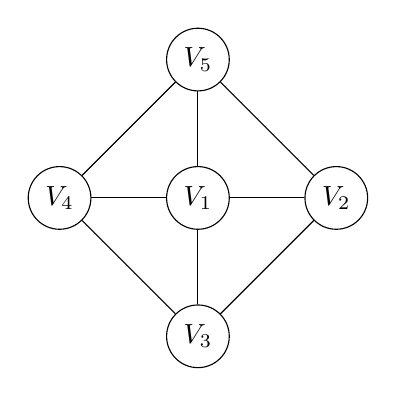
\begin{tikzpicture}[main/.style = {draw, circle}, node distance={50pt}]
                                    \node[main] (1) {$V_1$};
                                    \node[main] (2) [right of=1] {$V_2$};
                                    \node[main] (3) [below of=1] {$V_3$};
                                    \node[main] (4) [left of=1]  {$V_4$};
                                    \node[main] (5) [above of=1] {$V_5$};
                                    \draw (1) -- (2);
                                    \draw (1) -- (3);
                                    \draw (1) -- (4);
                                    \draw (1) -- (5);
                                    \draw (2) -- (3);
                                    \draw (3) -- (4);
                                    \draw (4) -- (5);
                                    \draw (5) -- (2);
                              \end{tikzpicture}
                        \end{center}

                        Este posibil să se aleagă pentru MST muchiile $(V_1, V_2), (V_1, V_3), \dots$:

                        \begin{center}
                              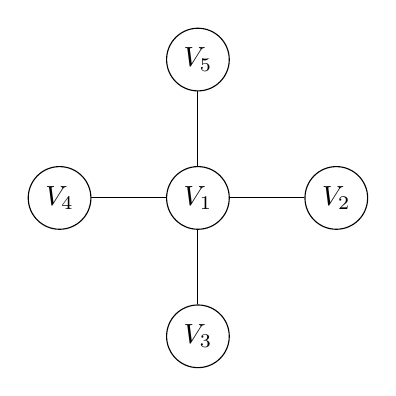
\begin{tikzpicture}[main/.style = {draw, circle}, node distance={50pt}]
                                    \node[main] (1) {$V_1$};
                                    \node[main] (2) [right of=1] {$V_2$};
                                    \node[main] (3) [below of=1] {$V_3$};
                                    \node[main] (4) [left of=1]  {$V_4$};
                                    \node[main] (5) [above of=1] {$V_5$};
                                    \draw (1) -- (2);
                                    \draw (1) -- (3);
                                    \draw (1) -- (4);
                                    \draw (1) -- (5);
                                    \draw (2) -- (1);
                              \end{tikzpicture}
                        \end{center}

                        Este posibil să se aleagă ca start $V_1$ și să se meargă în ordinea:
                        \[V_1, V_2, V_4, V_6, \dots, V_3, V_5, V_7, \dots\, V_1\].

                        Dar există soluție optimă doar cu muchii de cost $1$: \[V_1, V_2, V_3, \dots, V_n, V_1\].

                        \[\lim_{n \to \infty} \frac{\ALG}{\OPT} = \frac{1 + (n - 1) * 2 + 1}{n + 1} = 2\].

                        Deci factorul de aproximare 2 este tight-bound.
                        Deoarece $G_n$ are doar muchii de cost 1 sau 2, tight-bound-ul se aplică pentru
                        TSP cu muchii de cost 1 sau 2.

                        (Nu este specificat cum se alege MST-ul și nodul start.
                        Dacă este aleator, atunci e posibil să se aleagă soluția de cost $2n$.
                        Dacă alegerea e bazată pe ordinea nodurilor, i.e. se alege mereu turul
                        $V_1, V_2, V_3, \dots, V_n, V_1$, atunci se pot reordona nodurile pentru
                        a păcăli algoritmul să aleagă soluția de cost $2n$.)

            \end{enumerate}

\end{enumerate}

\section{Vertex Cover}

Fie $X = \{x_1, x_2, \dots, x_n\}$ o o mulțime de variabile boolene. Numim formulă
booleană (peste mulțimea $X$) în Conjunctive Normal Form (CNF) o
expresie de forma $C_1 \land C_2 \land \dots \land C_m$, unde fiecare $C_i$ este
o disjuncție a unui număr de variabile.

Ne interesează să aflăm numărul minim de variabile care trebuie să aibă valoarea
$true$ astfel încât expresia să fie $true$.

Fie următorul algoritm pentru problema de mai sus în varianta în
care fiecare clauză are exact trei variabile (numită 3CNF):

\subsection{Greedy-3CNF}

\begin{enumerate}
      \item
            Fie $C = \{C_1, C_2, \dots, C_m\}$ mulțimea de predicate,
            $X = \{x_1, x_2, \dots, x_n\}$ mulțimea de variabile.
      \item
            Cât timp $C \neq \emptyset$:
            \begin{enumerate}
                  \item Alegem aleator un $C_i \in C$.
                  \item Fie $x_j$ o variabilă din $C_i$.
                  \item $x_j \leftarrow true$.
                  \item Eliminăm din $C$ toate clauzele care conțin $x_j$.
            \end{enumerate}
      \item Soluția este mulțimea de variabile care au fost setate la $true$.
\end{enumerate}

\subsection{Cerințe}

\begin{enumerate}[label=\alph*)]
      \item (0,5p) Analizați factorul de aproximare (worst case) al algoritmului.

            %Fie $C_i = C_1 \lor C_2 \lor C_x \;\;\forall x \in [3, n], n = |X|$.

            \[\text{Fie}\ C = \bigwedge\limits_{i=3}^{n} (x_1 \lor x_2 \lor x_i)\]

            Este posibil ca algoritmul să aleagă variabilele \{$x_3, x_4, \dots, x_n$\},
            dacă alege mereu a treia variabilă din fiecare clauză,
            dar soluția optimă este $\{x_1\}$ sau $\{x_2\}$.

            $\lim_{n \to \infty} \frac{\ALG}{\OPT} = \lim_{n \to \infty} \frac{n - 2}{1} = \infty$.

            Soluția dată de algoritm poate fi arbitrar de rea, deci nu există un factor de aproximare.

      \item (0,5p) Modificați algoritmul de mai sus, astfel încât acesta să fie un algoritm 3-aproximativ
            pentru problema inițială (și justificați).

            În loc de a alege o singură variabilă, se aleg toate variabilele dintr-o clauza aleasă aleator.

            \subsubsection*{Demonstrație (similar cu cea de la curs)}

            Algoritmul este similar cu cel de la curs pentru Vertex Cover, dar muchiile au trei noduri în loc de două.

            \paragraph*{Lemă}

            Fie $C^*$ o mulțime de clauze disjuncte, fie $S$ o mulțime de variabile care rezolvă problema.
            $S$ trebuie să acopere toate clauzele din $C^*$.

            Fiecare variabilă din $S$ acoperă cel mult o clauză din $C^*$.
            Fie există o singură variabilă pentru fiecare clauză din $C^*$,
            fie unele clauze sunt acoperite de mai multe variabile.

            Deci $|S| = \OPT \geq |C^*|$.

            \paragraph*{Teorema}

            Fie $C^*$ mulțimea de clauze alese aleator de algoritm, $S$ mulțimea de variabile alese de algoritm.

            Deoarece la fiecare pas se elimină toate variabilele în comun cu clauza aleasă,
            $C^*$ este o mulțime de clauze disjuncte, deci $\OPT \geq |C^*|$.

            Pentru fiecare clauză aleasă, se adaugă $3$ variabile, deci $|S| = 3|C^*|$.
            Substituind în $\OPT \geq |C^*|$, obținem $\OPT \geq \frac{1}{3}|S|$.

            $3 \cdot \OPT \geq |S|$, deci algoritmul este 3-aproximativ.

      \item (0,5p) Reformulează problema de mai sus sub forma unei probleme de programare liniară (cu numere reale).

            Minimizăm $x_1 + x_2 + \dots + x_n$, folosind constrângerile generate din clauza $C$:

            \[\forall (x_1 \lor x_2 \lor x_3) \in C,\; x_1 + x_2 + x_3 \geq 1\]
            \[x_i \in [0, 1] \;\forall\; i \in \{1, 2, \dots, n\}\]

      \item (0,5p) Dați o soluție 3-aproximativă pentru problema de programare liniară formulată la sub-punctul anterior.

            Rulăm simplex pe problema de programare liniară formulată anterior.

            Pentru a converti soluția problemei de programare liniară în soluția problemei inițiale,
            se va seta $X_i \leftarrow \text{\it{true}}$ dacă și numai dacă $x_i \geq \frac{1}{3}$.

            Soluția $S$ aleasă va fi o soluție pentru clauză, deoarece
            $x_1 + x_2 + x_i \geq 1 \implies x_i \geq \frac{1}{3}\ \text{pentru cel puțin un}\ i$.

            \[
                  \ALG = \sum_{i=1}^{n}\begin{cases}
                        1, & x_i \geq \frac{1}{3} \\
                        0, & x_i < \frac{1}{3}
                  \end{cases}
                  \leq 3 \cdot \sum_{i=1}^{n} x_i
                  \leq 3 \cdot \OPT
            \]

\end{enumerate}

\end{document}
